\documentclass{acmsiggraph}                     % final
%\documentclass[annualconference]{acmsiggraph}  % final (annual conference)
%\documentclass[review]{acmsiggraph}            % review
%\documentclass[widereview]{acmsiggraph}        % wide-spaced review
%\documentclass[preprint]{acmsiggraph}          % preprint

%% Uncomment one of the five lines above depending on where your paper is
%% in the conference process. ``review'' and ``widereview'' are for review
%% submission, ``preprint'' is for pre-publication, and ``final'' is for
%% the version to be printed. The ``final'' variant will accept the 
%% ``annualconference'' parameter, which changes the height of the space
%% left clear for the ACM copyright information.

%% The 'helvet' and 'times' packages define the typefaces used for
%% serif and sans serif type in this document. Computer Modern Roman 
%% is used for mathematics typesetting. The scale factor is set to .92
%% to bring the sans-serif type in line with the serif type.

\usepackage[scaled=.92]{helvet}
\usepackage{times}

%% The 'graphicx' package allows for the inclusion of EPS figures.

\usepackage{graphicx}

%% use this for zero \parindent and non-zero \parskip, intelligently.

\usepackage{parskip}

%% Optional: the 'caption' package provides a nicer-looking replacement
%% for the standard caption environment. With 'labelfont=bf,'textfont=it',
%% caption labels are bold and caption text is italic.

\usepackage[labelfont=bf,textfont=it]{caption}

%% If you are submitting a paper to the annual conference, please replace 
%% the value ``0'' below with the numeric value of your OnlineID. 
%% If you are not submitting this paper to the annual conference, 
%% you may safely leave it at ``0'' -- it will not be included in the output.

\onlineid{0}

%% Paper title.

\title{A Study of Immersion Factors Using an Augmented Reality Simulation}

%% Author and Affiliation (single author).

%%\author{Roy G. Biv\thanks{e-mail: roy.g.biv@aol.com}\\Allied Widgets Research}

%% Author and Affiliation (multiple authors).

\author{
%Roy G. Biv\thanks{e-mail: roy.g.biv@aol.com}\\ Starbucks Research %
%\and Ed Grimley\thanks{e-mail:ed.grimley@aol.com}\\Nigel Mansell\thanks{nigelf1@msn.com}\\ Grimley Widgets, Inc. %
%\and Martha Stewart\thanks{e-mail:martha.stewart@marthastewart.com}\\ Martha Stewart Enterprises \\ Microsoft Research}
}

%% Keywords that describe your work.

\keywords{
%radiosity, global illumination, constant time
}

%%%%%% START OF THE PAPER %%%%%%

\begin{document}

%\teaser{
%  \includegraphics[width=1.5in]{sample.eps}
%  \caption{Lookit! Lookit!}
%}

%% The ``\maketitle'' command must be the first command after the
%% ``\begin{document}'' command. It prepares and prints the title block.

\maketitle

%% Abstract section.

\begin{abstract}
It is extremely challenging to run controlled studies comparing multiple augmented reality (AR) systems.  We use an �AR simulation� approach, in which a virtual reality (VR) system is used to simulate multiple AR systems. In order to validate this approach, we carefully replicated a well-known study by Ellis et al. using our simulator, obtaining comparable results. 

In a second study using the AR simulator, we studied a tracking task where the AR interface provides x-ray vision to help track a moving target.  We varied the field of view of the AR display, as well as the reliability of the head tracker.  In low reliability conditions, we simulate tracker failure by disabling the augmented view of the scene for brief periods.  Our study gives insight into the effect of head tracker reliability on user performance in a tracking task, as well as the relationship between reliability and field of view in an AR system.

\end{abstract}

%% ACM Computing Review (CR) categories. 
%% See <http://www.acm.org/class/1998/> for details.
%% The ``\CRcat'' command takes four arguments.

\begin{CRcatlist}
%  \CRcat{K.6.1}{Management of Computing and Information Systems}{Project and People Management}{Life Cycle};
%  \CRcat{K.7.m}{The Computing Profession}{Miscellaneous}{Ethics}
\end{CRcatlist}

%% The ``\keywordlist'' command prints out the keywords.
\keywordlist

\section{Introduction}

%% The ``\copyrightspace'' command must be the first command after the 
%% start of the first section of the body of your paper. It ensures the
%% copyright space is left at the bottom of the first column on the first
%% page of your paper.

%% \copyrightspace

motivation??

\section{Related Work}

Livingston and Ai studied the effects of various sources of registration error with an AR simulation similar to our own.  Here, participants tracked a virtual car moving throughout a real environment, with a white box representing an augmented view of the car's location.  A white box was continuously visible, even when the car itself was occluded by a building in the environment.  Other virtual cars and their associated white boxes acted as distractors.  At specific times during the experiment, the simulation would freeze and the participant was asked to align the center of their view (indicated by cross-hairs) on the location of the correct car and press a key.  While the effects of several types of error were studied in this work, the effect of registration dropouts was not examined.

other studies which vary AR fov, tracking failures

previous X-ray AR work

simulated AR

\cite{4637329,4811058,1383060}

\section{AR Simulator Validation}

Cha's text goes here

\subsection{Experimental Design}

\begin{figure}[ht!]
	\centering
	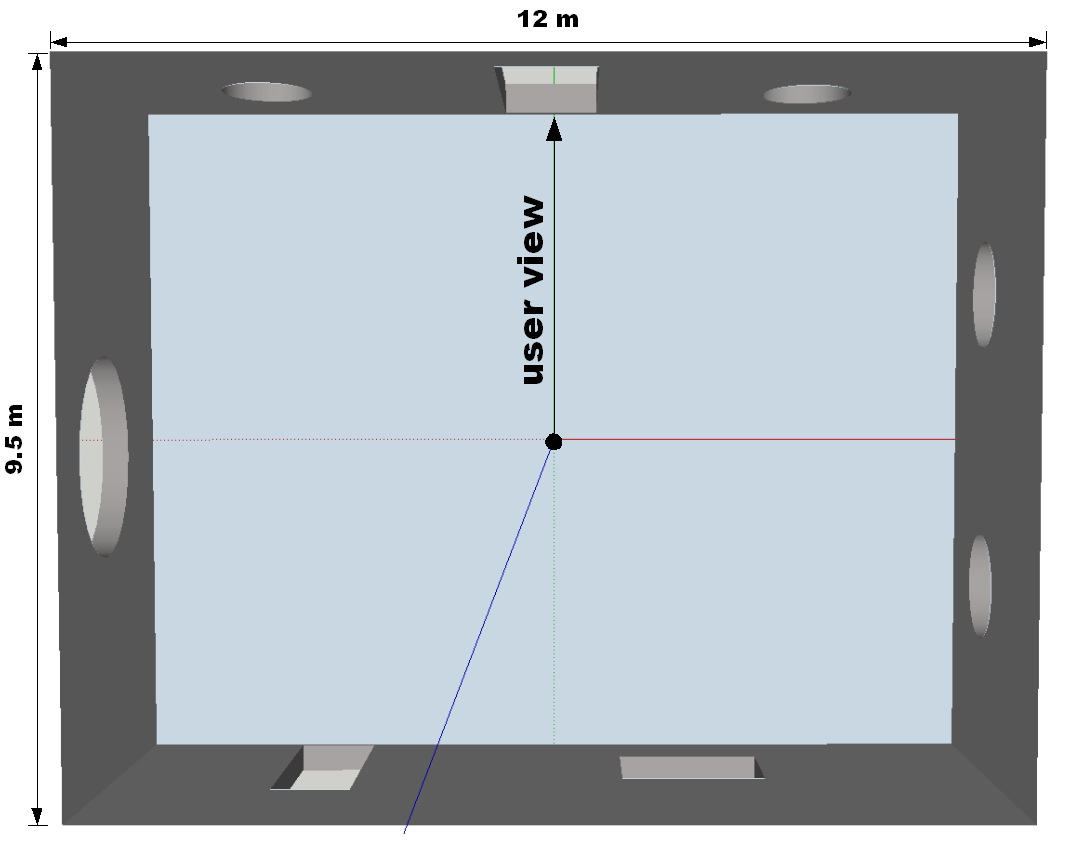
\includegraphics[width=3.5in]{annotated_room.png}
	\caption{Overhead view of virtual room (approx. measure)}
\end{figure}


\subsection{Results}

\subsection{Analysis}

\section{Tracking Study}

Our experiment involves a tracking task which uses an augmented reality interface to allow people to be tracked behind walls.  A participant stands in the middle of a square room with doors and windows on all sides.  Outside of the room, people are walking around the building.  The target person to be tracked is visually distinguishable by a large black top hat.  The augmented reality interface overlays a translucent red rectangle on each person, which is visible even when the person is occluded by a wall.  However, the target person's overlay is not different from any other person's overlay; the target is only identifiable when visible through a window or a door.

To actually run this experiment using a true augmented reality system would be difficult.  Many confederates would be needed to walk around the room, and their movements would need to be accurately reproduced for each new participant.  Also, the confederates would need to be continously tracked for the augmented overlays to be displayed.  Instead, we simulated the experiment setup in a completely virtual environment.

By simulating augmented reality, we are freed from the current restrictions of tracking and display technology.  Using a simulated environment also makes the experiment more controllable, and thus more easily reproduced.

\subsection{Experimental Design}
Participants are presented a view of the scene through a head-mounted display helmet with orientation tracking.  The tracking overlays are  augmented on top of the image to form the simulated augmented reality view.

The parameters of our experiment are divided between the ``real'' immersion factors, such as the field of view of the HMD, and the ``augmented'' immersion factors, such as the field of view of the simulated AR display, and the performance of the head tracker.  We introduce periods of tracking failure, where the augmented overlays disappear, to simulate the effect of failures in a real tracking system.  For example, such failures might occur with a magnetic tracker near interfering materials, or with visual tracking when tracked features are lost.

In our experiment we vary two parameters: the field of view of the AR interface and the length of tracking failure periods.  Each trial lasted sixty seconds, and had seven tracking failures.  The total vertical field of view of our HMD is 36 degrees; the three possible values for the augmented field of view were 10, 20, and 34 degrees.  We varied the length of tracking failures between two seconds, one second and zero seconds (no failure).

\subsection{Results}

\subsection{Analysis}

\section{Conclusions and Future Work}

\section*{Acknowledgements}

\bibliographystyle{acmsiggraph}
\nocite{*}
\bibliography{paper}
\end{document}
